
\documentclass [a4paper]{tufte-book}\usepackage[]{graphicx}\usepackage[]{color}
%% maxwidth is the original width if it is less than linewidth
%% otherwise use linewidth (to make sure the graphics do not exceed the margin)
\makeatletter
\def\maxwidth{ %
  \ifdim\Gin@nat@width>\linewidth
    \linewidth
  \else
    \Gin@nat@width
  \fi
}
\makeatother

\usepackage{Sweavel}


\usepackage{color}
\usepackage{xcolor}
\usepackage{framed}
\usepackage{listings}

\usepackage{graphicx}

\usepackage{multicol}              
\usepackage{multirow}
\usepackage{booktabs}
%\usepackage{natbib} 

\usepackage[innerrightmargin = 0.7cm, innerleftmargin = 0.3cm]{mdframed}
\usepackage{mdwlist}

\usepackage[]{hyperref}
\definecolor{darkblue}{rgb}{0,0,.5}
\hypersetup{colorlinks=true, breaklinks=true, linkcolor=darkblue, menucolor=darkblue, urlcolor=blue, citecolor=darkblue}

\usepackage[toc,page]{appendix}


\setcounter{secnumdepth}{1}
\setcounter{tocdepth}{1}

\lstset{ % settings for listings needs to be be changed to R sytanx 
language=R,
breaklines = true,
breakautoindent = false,
basicstyle=\ttfamily \scriptsize,
keywordstyle=\color{black},                          
identifierstyle=\color{black},
commentstyle=\color{gray},
xleftmargin=3.4pt,
xrightmargin=3.4pt,
numbers=none
}

%\VignetteIndexEntry{PhylGeo}
%\VignetteEngine{knitr::knitr}



\title{PhyloSim Package\\ Vignette}

\author{}
\begin{document}
\maketitle
\tableofcontents
\chapter{Introduction}
The question whether or to which degree on can infer community assembly processes from their resulting spatial and phylogenetic patterns is of central importance in ecology. It is these processes that create and maintain local assemblages.\\
Currently there are many different explanations as to how species communities are shaped based on the emerging spatial or phylogenetic patterns. 
The phylosim package represents an expansion of previous models by combining these informations.\\
The simulation can include different mechanisms of community assembly such as dispersal limitation, environmental preferences and local competition, whereas the outcome consists of phylogenetic and spatial patterns. The mechanisms can be activated seperately or in combination. This allows the user to identify biogeographic or phylogenetic patterns exclusively correlated with a certain mechanism or combination of mechanisms.\\
Among the central model the package comprises a set of functions to illustrate and analyze the results.


\chapter{The model}
\section{The grid}
The basis for the simualtion is a grid of spatially discrete cells.
Each cell is inhabited by one individual at any time. Additionally an environmental gradient can be included. To avoid boundary effects the boundaries of the grid are warped.

\section{The indivuduals}
Each individual belongs to a species. The properties of the individual are represented in two traits ranging between zero and one.
The competition trait represents the individual's preferences apart from the environment. The more similar the traits of two individuals, the stronger they compete with each other.\\
The environmental trait simulates the individual's interaction with the environment. 
It is defined as the mean of a Gaussian Distribution with $\sigma$ set to 0.047. This represents a niche width covering ten percent of the total space of the
respective resource (approch see: \citep{ackermann2004}).\\ Further ech individual
possesses a neutral trait. This trait evolves over time but is influencing the individual's properties.\\
Apart from the individual's traits each species has trait values. These traits are not independent but defined as the mean of the respective traits of all individuals of the species. 
The species traits serve as an attractor in the individual trait evolution proces.
Further, each species contains information about its parent species and the species that emerged from it. 

\section{Processes}
The simulation runs over a defined number of generations. 
In each generation the simulation consists of three consecutive steps.\\
First the individuals reproduce and spread over the grid. All cells are sequentially chosen at random and the individuals are replaced by the offspring of other individuals.\\
The individual which produces its offspring and disperses into an empty cell is chosen by an multinomial distribution which consists of all cells within the dispersion kernel.
The dispersion kernel represents the distance to the cell to be populated and is defined as:
\begin{equation}
w_d = exp\frac{1}{-\Delta_s/2}
\end{equation}
$w_d$ represents the weight weight derived from the euclidean distance $\Delta_s$ between the
cell to be populated and the potential parent. An increasing distance to the cell leads to an exponential decline in reproductive fitness. The dispersal kernel can be cut at a certain radius.\\
The density dependence is based on the competition traits of the indivuduals. The closer the values of the competition traits of two individuals, the stronger they compete. Numerically it can be written as the sum of all absolute competition trait differences in a certain area around the individual. The normalized value is now included in the multinomial distribution as follows:
\begin{equation}
r_i = \frac{\sum_{j=1}^{n}{\parallel(c_i-c_j)}\parallel}{n}
\end{equation}
The second step in the simulation of one generation is the trait evolution. This step represents genetic recombination in the real world.
The trait is modelled as the mean of a Gaussian Distribution (see above). In each generation this value is slightly changed. The new trait is influenced by the parent's value, a weighted random value and the attraction of the specie's value. The parent value has the highest influence whereas the other two traits have only slight influence.
The trait values during trait evolution are calculated as follows:
\begin{equation}
newtrait = (1-w_s \cdot p) + (w_s \cdot s) + (w_r \cdot r)
\end{equation}

The last step in a generation is speciation. Here it describes the introduction of a new species via point mutations. These mutations can either become more abundand or go extinct \citep{hubbell1997}.The frequency of these events is controlled by the speciation rate in the parameter settings. Each generation a number of new species is introduced in the system replacing randomly chosen individuals. The traits of these individuals are calculated from the parent's traits and a randomly generated value as follows:
\begin{equation}
newtrait = (w_p \cdot p) + (w_r \cdot r)
\end{equation}


\chapter{Basic functionality}

\section{Summary}
The following section descibes how the model is applied and shows some of the most important funktions to illustrate and analyze the results of the simulations.\\
The basic structure of how the model is applied is shown in figure \ref{fig: func}.
\begin{figure}[h]
	\centering
	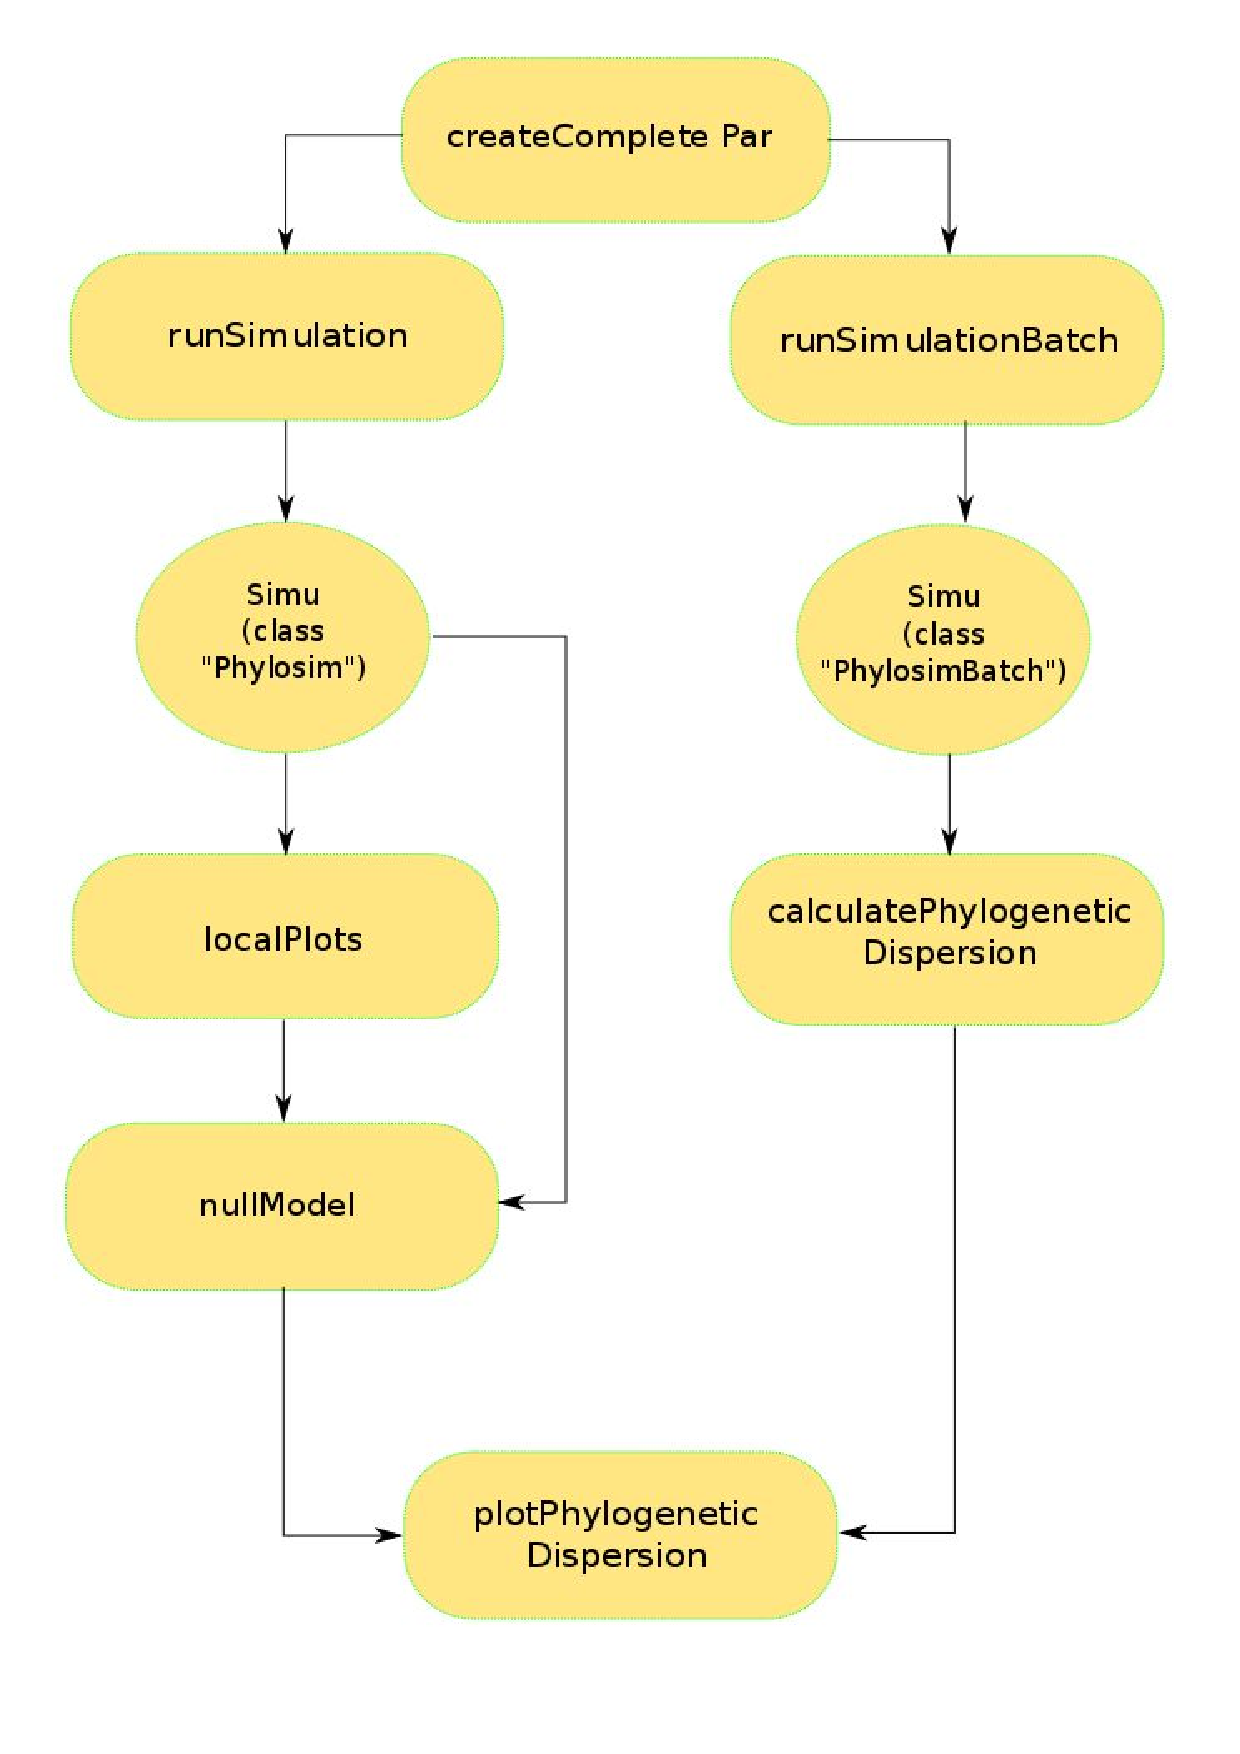
\includegraphics[width=12cm]{flowchart} % without file extension
	\caption{Overview about the basic functions in the Phylosim package}\label{fig: func}
\end{figure} 
\FloatBarrier




\section{Loading the package}

Loading the package via

\begin{Schunk}
\begin{Sinput}
library(PhylGeo)
\end{Sinput}
\begin{Soutput}
Warning: package 'foreach' was built under R version 3.2.2
\end{Soutput}
\end{Schunk}


\section{Run the model}
Running the model consists of two consecutive steps. First a list of parameters is generated based on the users settings.\\
In the following example an area of 50*50 cells provides the basis for one simulation with 1000 generations. Also the results after 500 generations will be stored in the output. \\
The dispersal is set to global, meaning each individual could reproduce in every cell
of the grid. Further, the density as well as the environment have an influence on the 
individuals.\\
The package can run three types of models. The default model, a Leipzig model and
a neutral model purely written in R. The last one is to be seen only for test and teaching purpose. To be used in practice it is far too slow.

For further explanations and more settings see:
\begin{Schunk}
\begin{Sinput}
?createCompletePar
\end{Sinput}
\end{Schunk}

\begin{Schunk}
\begin{Sinput}
par <- createCompletePar(x = 50, y = 50, dispersal = "global" , runs = c(500,1000), density = 1, environment = 0.5, specRate = 1, type="base")
\end{Sinput}
\end{Schunk}



The list of parameters is now being used to exectute the simulation:
\begin{Schunk}
\begin{Sinput}
simu <- runSimulation(par)
\end{Sinput}
\end{Schunk}


The output is saved as an object of type "Phylosim".
Each Phylosim object consists of two lists, \$Output and \$Model.
All model results are saved in the Output list. In this example the
Output consists of two results, the simulation after 500 and 1000 generations.
To acces them the easiest way is to use indexes.
\begin{Schunk}
\begin{Sinput}
Output1 <- simu$Output[[1]]
\end{Sinput}
\end{Schunk}
There are several objects in this list.
\begin{Schunk}
\begin{Sinput}
str(Output1)
\end{Sinput}
\begin{Soutput}
List of 7
 $ specMat  : int [1:50, 1:50] 290 419 429 419 429 290 419 163 290 419 ...
 $ traitMat : num [1:50, 1:50] 0.54 0.559 0.486 0.557 0.479 ...
 $ envMat   : num [1:50, 1:50] 0 0 0 0 0 0 0 0 0 0 ...
 $ compMat  : num [1:50, 1:50] 0.642 0.656 0.355 0.674 0.352 ...
 $ neutMat  : num [1:50, 1:50] 0.582 0.558 0.492 0.541 0.5 ...
 $ phylogeny:List of 6
  ..$ edge       : int [1:33, 1:2] 19 20 21 21 22 23 24 25 25 24 ...
  ..$ Nnode      : int 16
  ..$ tip.label  : chr [1:18] "s1" "s163" "s512" "s510" ...
  ..$ edge.length: num [1:33] 6 40 199 260 21 57 2 4 4 6 ...
  ..$ node.label : chr [1:16] "s1" "s1" "s1" "s163" ...
  ..$ root.edge  : num 110
  ..- attr(*, "class")= chr "phylo"
  ..- attr(*, "order")= chr "cladewise"
 $ phyloTXT : chr "(((s1:199,((((s163:4,s512:4)s163:2,s510:6)s163:57,s455:63)s163:21,s429:84)s163:260)s1:40,s120:384)s1:6,((((s114:141,s366:54)s11"| __truncated__
\end{Soutput}
\end{Schunk}
These are the species matrix, the (environmental) trait matrix, the environmental matrix (representing the environment), the competition matrix and the neutral matrix as well as the phlogeny in two formats.\\
The parameter settings are only saved once. Additionaly, the run time is saved with these settings.
\begin{Schunk}
\begin{Sinput}
str(simu$Model)
\end{Sinput}
\begin{Soutput}
List of 16
 $ x                        : num 50
 $ y                        : num 50
 $ dispersal                : chr "global"
 $ runs                     : num [1:2] 500 1000
 $ specRate                 : num 1
 $ density                  : logi TRUE
 $ environment              : logi TRUE
 $ fitnessActsOn            : chr "mortality"
 $ fitnessBaseMortalityRatio: num 10
 $ densityCut               : num 1
 $ seed                     : int 2863
 $ type                     : chr "base"
 $ scenario                 : NULL
 $ compStrength             : num 1
 $ envStrength              : num 0.5
 $ runtime                  : num 2.34
\end{Soutput}
\end{Schunk}


In the package, the Phylosim object serves as the basis of all further analysis.
It can directly be passed to all other funktions.
If the Phylsim object contains multiple results, they can be accessed by the which.simulation argument. By default always the last result is used.\\
Because the simulations have a high computational cost, the package comprises a funktion to make use of parallel computing. This function can be seen as an extension to the
runSimulation funktion in order to accelerate the simulation of multiple scenarios.\\
As input serves a list of parameter settings as created by createCompletePar, whereas the output is a list of Phylosim objects.\\
In the following example two slightly different parameter sets are created and processed using parallel computing.

\begin{Schunk}
\begin{Sinput}
par1 <- createCompletePar(x = 50, y = 50, dispersal = "global", runs = 1000, density = 1, environment = 0.5, specRate = 1, type="base")

par2 <- createCompletePar(x = 50, y = 50, dispersal = "global", runs = 1000, density = 1, environment = 2, specRate = 1, type="base")

parmBatch <- list(par1, par2)

simuBatch <- runSimulationBatch(parmBatch, parallel = "auto")
\end{Sinput}
\end{Schunk}

The simuBatch object contains two Phylosim objects saved in a list. You can easily access them seperately by indexing. For example:

\begin{Schunk}
\begin{Sinput}
simu1 <- simuBatch[[1]]
\end{Sinput}
\end{Schunk}




\section{Plots and summary statistics}
\begin{figure}[h]
	\centering
	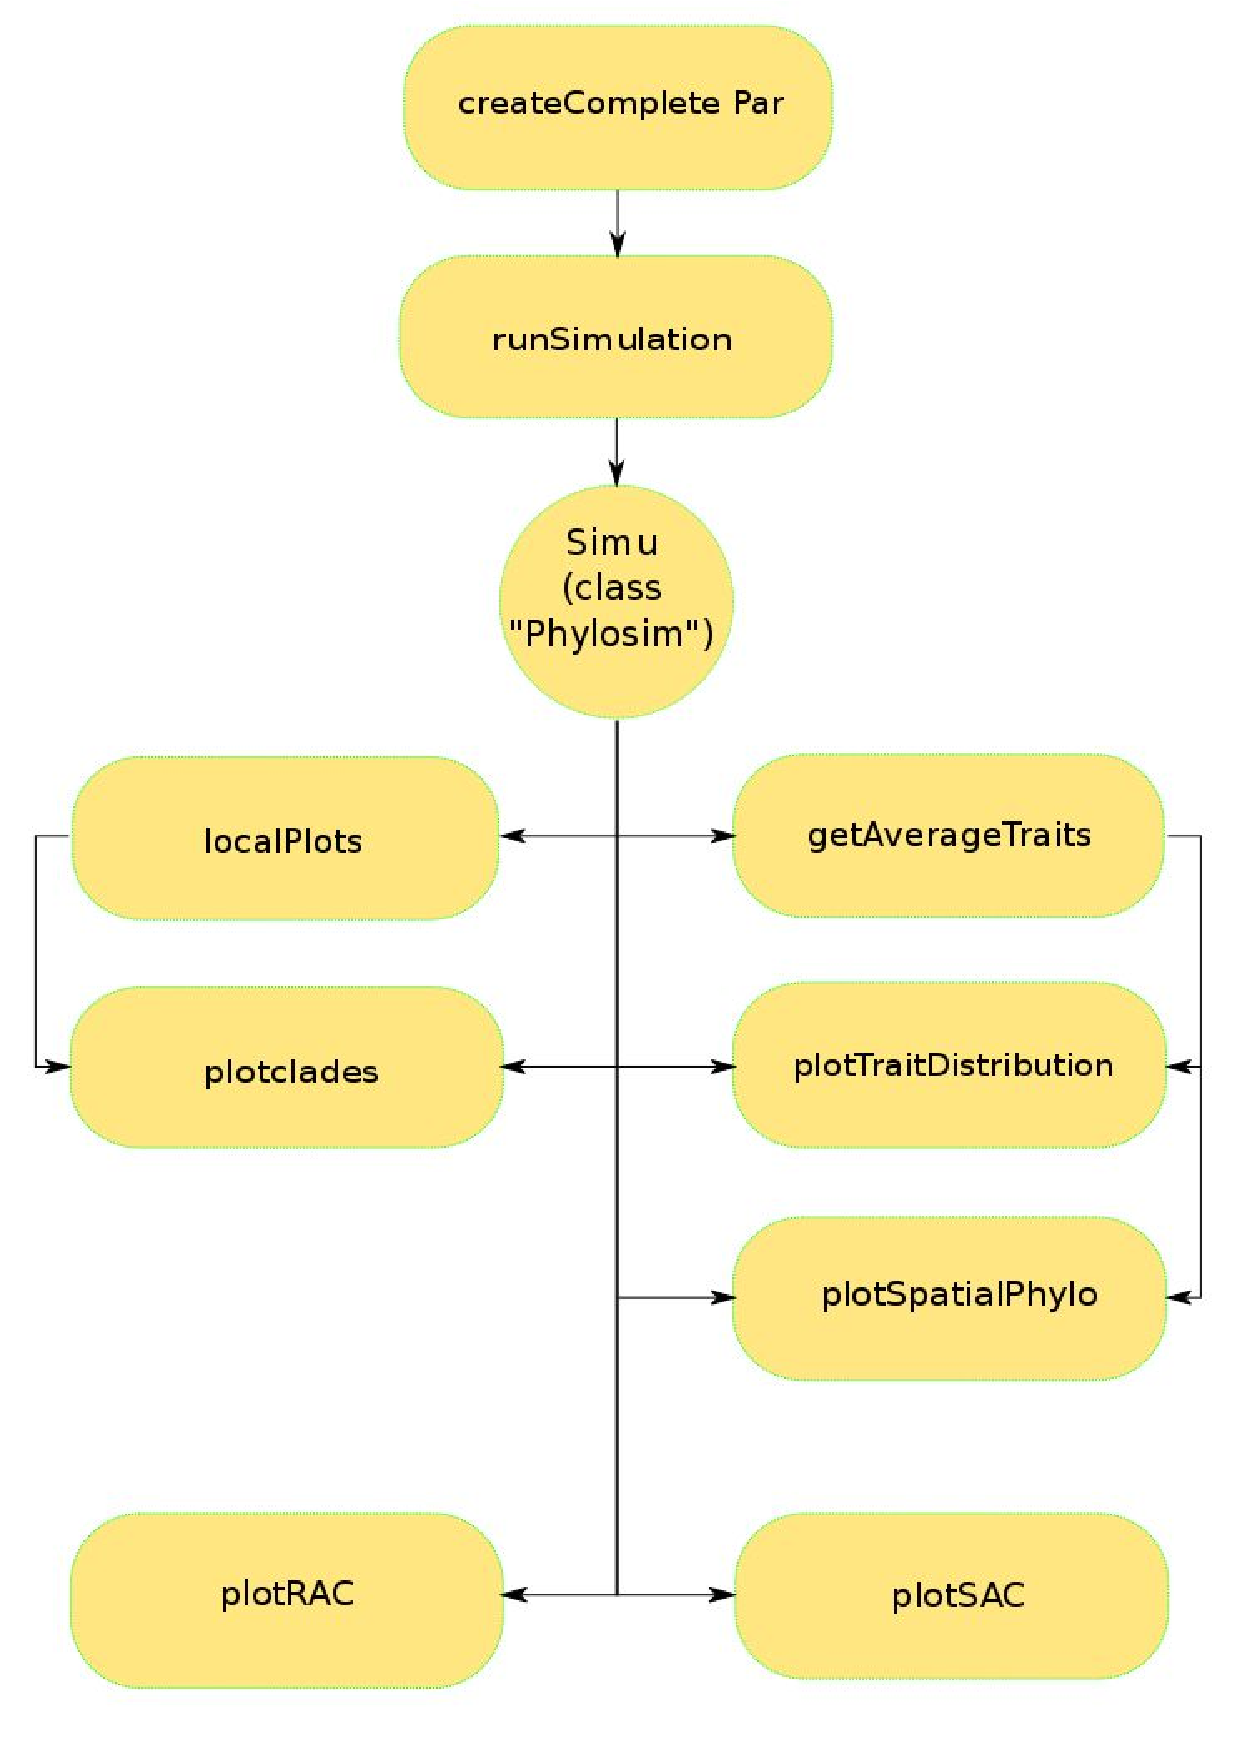
\includegraphics[width=12cm]{flowchart_plots} % without file extension
	\caption{Overview about the plotting functions in the Phylosim package}\label{fig: plots}
\end{figure} 
\FloatBarrier
The phylosim package contaions multiple functions to visualize the results of the simulation.
The plotSpatialPhylo plot consist of three different figures. The phylogeny tree that shows the phylogeny of the modeled community with colored tip labels. A traitplot that shows the magnitude of different traits for each of the species within the community. And a plot that shows the spatial abundance of the species within the community. Here the species have the same color as the tip labels for recognition. Which of these figures are plotted can be triggered with the arguments "plot" and "plotTraits" (see help).\\

\begin{Schunk}
\begin{Sinput}
plotSpatialPhylo(simu, plot = "both", plotTraits = T, which.simulation = NULL)
\end{Sinput}

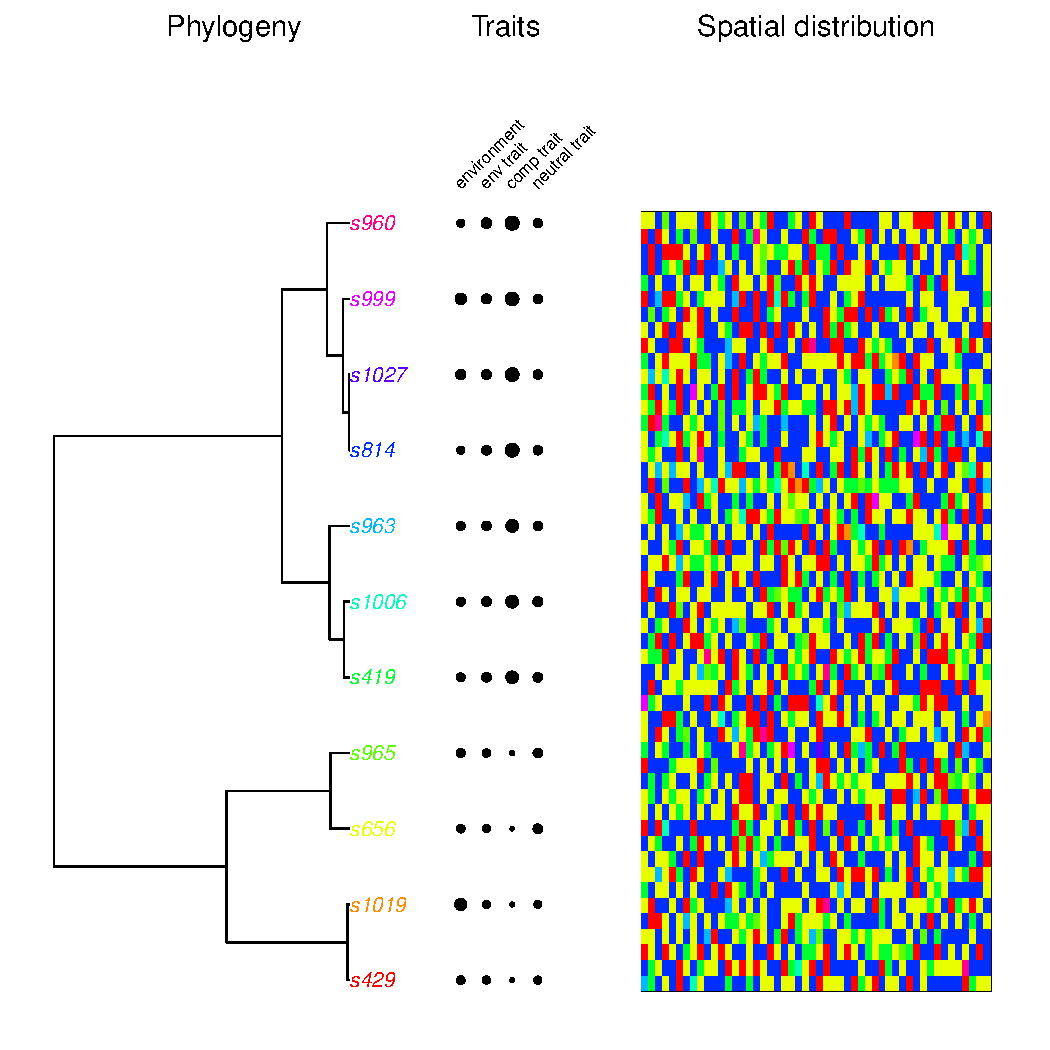
\includegraphics[width=\maxwidth]{figure/unnamed-chunk-10-1} \end{Schunk}


The plotTraitDistribution plot consists of three different figures for the three traits in the model (environmental trait, competition trait, neutral trait). Figure one illustrates the trait's magnitude in dependency of the environment for different species. Figure two illustrates the spatial distribution of the given trait. Figure three shows a histogram of the given trait.

\begin{Schunk}
\begin{Sinput}
plotTraitDistribution(simu = simu, which.simulation = NULL, type ="all")
\end{Sinput}

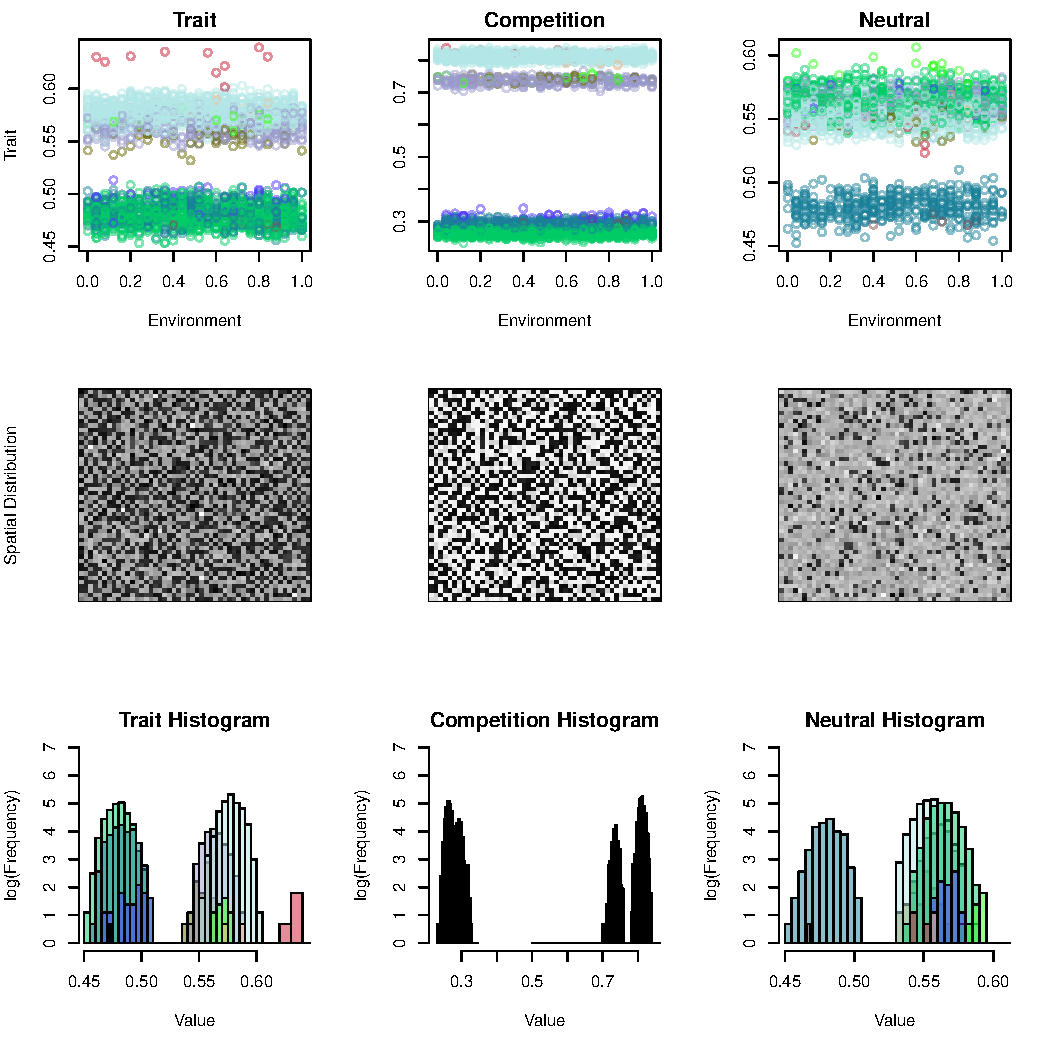
\includegraphics[width=\maxwidth]{figure/unnamed-chunk-11-1} \end{Schunk}

The package contains two functions to analyze the spatial patterns of the results.
The species-area curve (SAC) and the rank-abundace curve (RAC).
The SAC shows the accumulated species richness as a function of the plot size. 
A positively bent curve indicates clustering of a species community. An increase in plot size leads to an increase in specis richness. A negatively bent curve indicates a more neutral distribution of species within the community.\\
\begin{center}
\begin{Schunk}
\begin{Sinput}
sac(simu, which.simulation = NULL)
\end{Sinput}

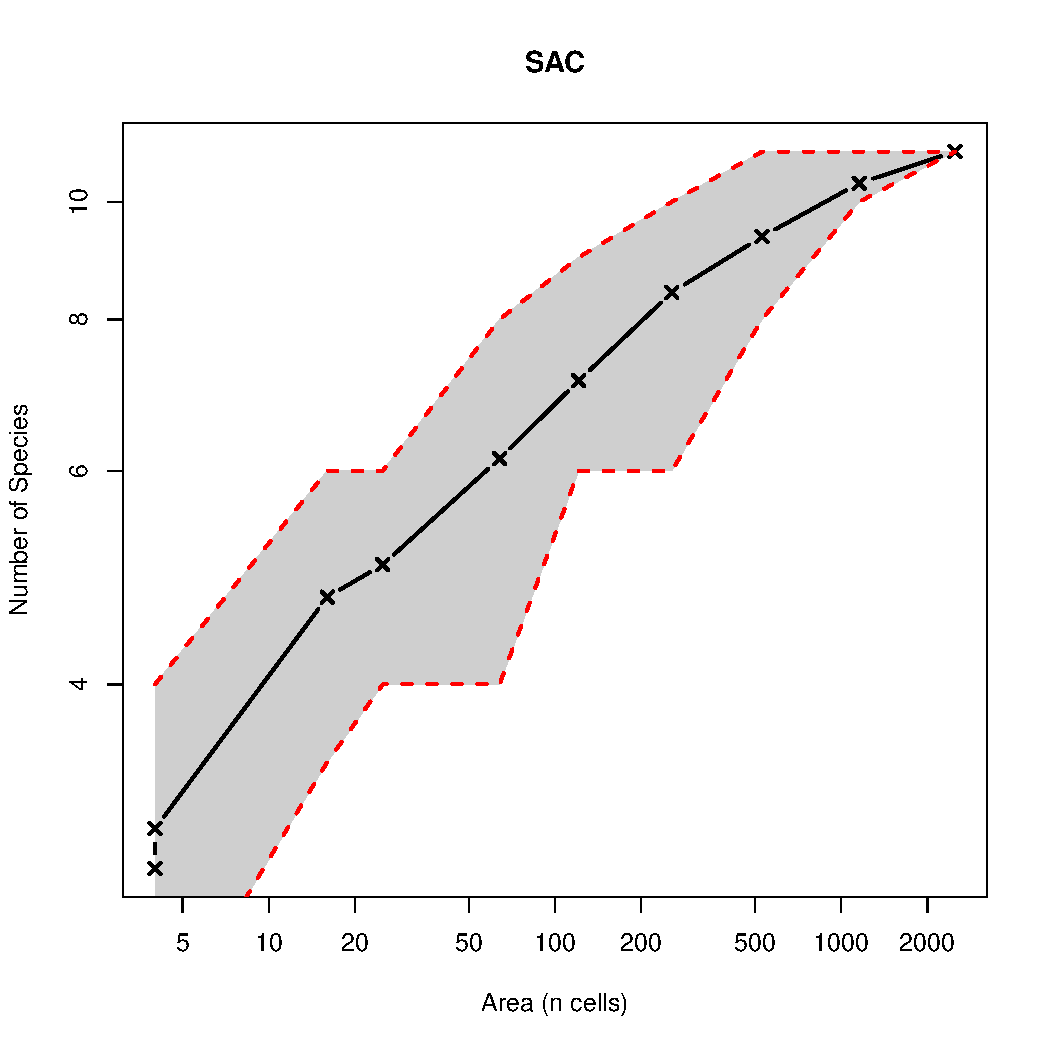
\includegraphics[width=6cm,height=6cm]{figure/unnamed-chunk-12-1} \end{Schunk}
\end{center}
RACs display the amount of equally abundand species that the community can support. A linear curve indicates a less stable or neutral community supporting only a few highly abundand species, whereas an S-shaped curve indicates a more stable community. In the latter case several species of the same abundance can be supported.\\

\begin{center}
\begin{Schunk}
\begin{Sinput}
rac(simu, which.simulation = NULL)
\end{Sinput}

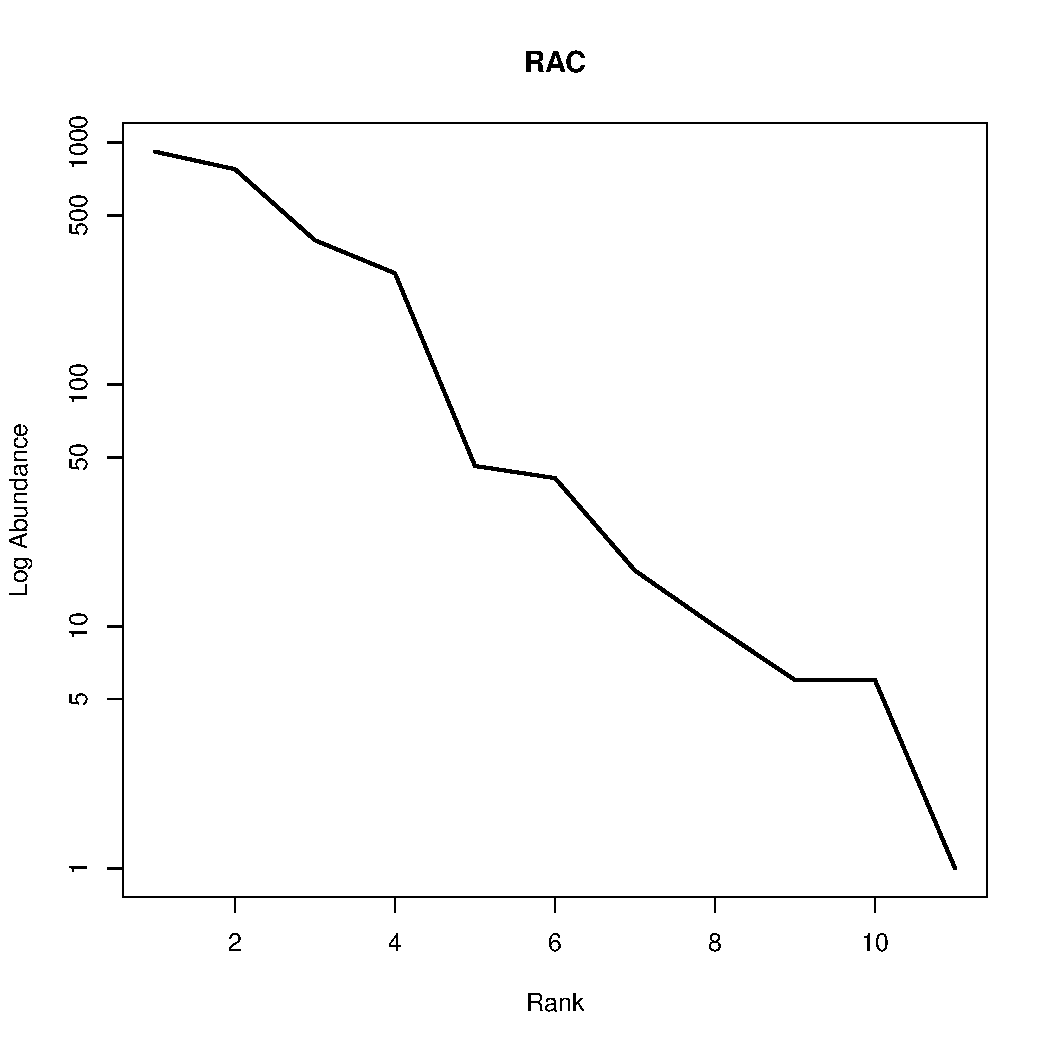
\includegraphics[width=6cm,height=6cm]{figure/unnamed-chunk-13-1} \end{Schunk}
\end{center}

As mentioned above each individual has a neutral trait. This trait evolved over time but is not influencing the individual's fitness.\\
However, these traits can be used to construct a phylogeny for a given community.
In the package this is implemented in the phlyoReconstruct function. \\
These phylogenies can now be compared to the real phylogeny of the community.
\begin{Schunk}
\begin{Sinput}
rePhyl <- phyloReconstruct(simu)
par(mfrow=c(1,2))
plot(rePhyl, main="reconstructed Phylogeny")
plot(simu$Output[[2]]$phylogeny, main="real Phylogeny")
\end{Sinput}

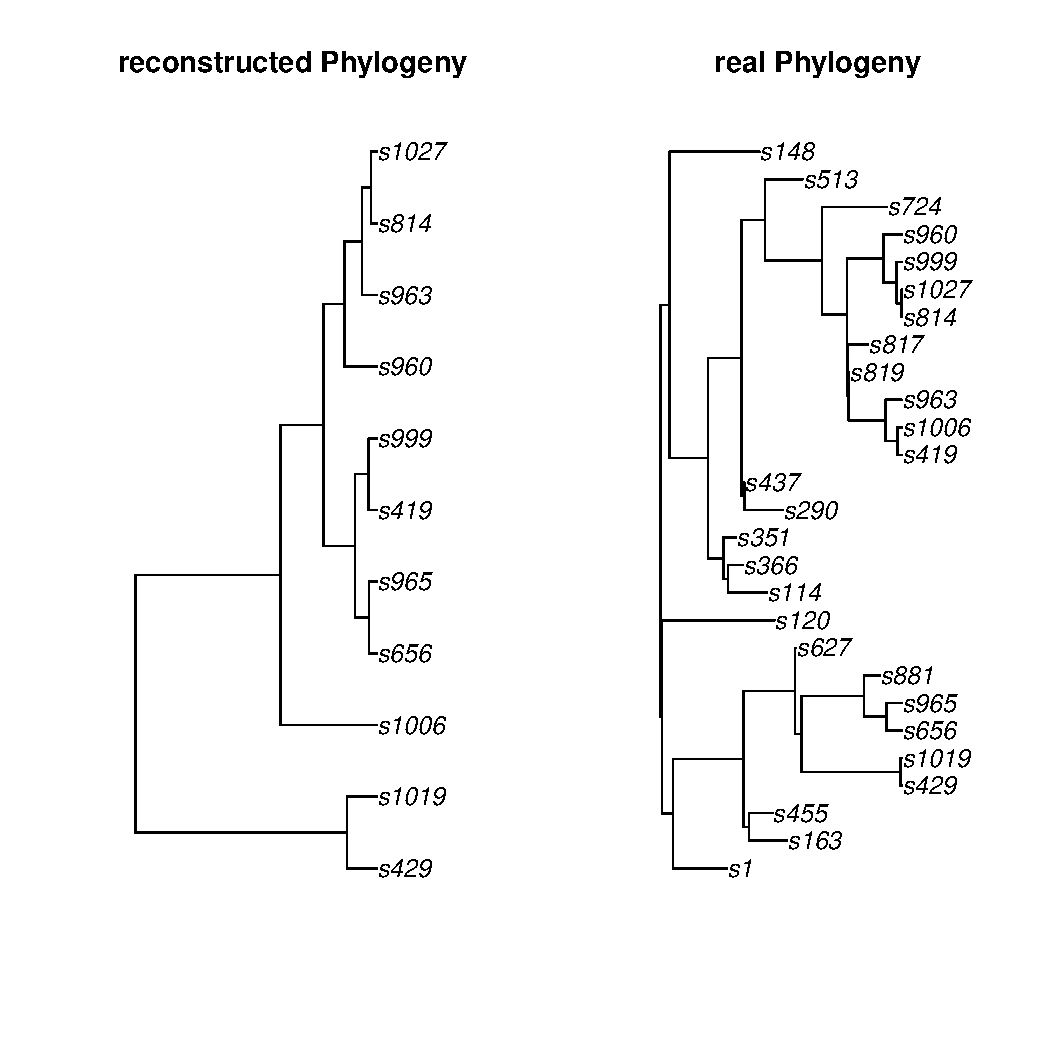
\includegraphics[width=\maxwidth]{figure/unnamed-chunk-14-1} \end{Schunk}


\chapter{Null Models}

To tackle the question, whether there are pattern in the results of the 
simualtions, the package comprises a set of null models to test the observed results
against. These models are brought together in the nullModel function.\\
In the function subplots of the results are created based on a Phylosim object.
These subplots can also be created seperately for different purposes.
\begin{Schunk}
\begin{Sinput}
subPlots <- localPlots(simu = simu, size=100, n=10)
\end{Sinput}
\end{Schunk}

These subplots are now tested against randomly collected plots.\\
You can choose, whether the null model should be based on the abundance distribution of the sample plots or not.\\
If the model is not based on the abundance distribution, there are two possible measures of the phylogeny that are used to compare the observed results to the null model. These are the Mean Pairwise Distance (mpd) or Fait's Phylogenetic Diversity (pd)\marginnote{the Mean Pairwise Distance and Fait's Phylogenetic Diversity have their origin in the picante package. For more information see the help pages in the picante package.}.

\begin{Schunk}
\begin{Sinput}
pValues <- nullModel(simu = simu, abundance = FALSE, localPlotSize = 100, numberOfPlots = 10, repetitions = 100, fun="mpd")
\end{Sinput}
\end{Schunk}

To analyze large outputs as created by runSimulationBatch the calculatePhylogeneticDispersion function can be useful. It can be seen as an extension to the nullModel function that deals with lists of Phylosim objects and can also calculate two external null models. Which null model is used is determined by the types argument with the following options.
\begin{itemize}
\item "PhylMeta" equivalent to the nullModell function with abundace = FALSE
\item "PhylSample"  equivalent to the nullModell function with abundace = TRUE
\item "PhylPool" uses picante::ses.mpd with null.model = "phylogeny.pool"
\item "SamplePool" uses picante::ses.mpd with null.model = "sample.pool"
\end{itemize}

\begin{Schunk}
\begin{Sinput}
pValuesBatch <- calculatePhylogeneticDispersion(simuBatch, plotlength=20, plots=20, replicates=20, types="PhylMeta")
\end{Sinput}
\end{Schunk}

\newpage

\bibliographystyle{chicago} 

\bibliography{Vignette_bib}





\end{document}
